\documentclass[12pt,a4paper]{article}

% --- Page Layout & Dimensions (Clean 1-inch margins) ---
\setlength{\textwidth}{6.5in}
\setlength{\textheight}{9.35in}
\setlength{\oddsidemargin}{0.0in}
\setlength{\evensidemargin}{0.0in}
\setlength{\topmargin}{-0.55in}
\setlength{\headheight}{0.0in}
\setlength{\headsep}{0.0in}
\setlength{\footskip}{26pt}
\setlength{\parindent}{0pt}
\setlength{\parskip}{0.56em}
\renewcommand{\baselinestretch}{1.08}

% --- Packages ---
\usepackage{mathptmx}  % Times New Roman font (Scalable Type 1 with math support)
\usepackage{graphicx}
\usepackage{url}
\usepackage{hyperref}
\usepackage{multirow}

% --- Itemize Bullets & Spacing ---
\renewcommand{\labelitemi}{$\bullet$}
\renewcommand{\labelitemii}{--}
\makeatletter
\def\@listi{\leftmargin\leftmargini
            \parsep 1\p@ \@plus\p@ \@minus\p@
            \topsep 3\p@ \@plus\p@ \@minus\p@
            \itemsep 1.5\p@ \@plus\p@ \@minus\p@}
\let\@listI\@listi
\makeatother

% --- Math & Helper Macros ---
\providecommand{\text}[1]{\mbox{#1}}
\providecommand{\mathbf}[1]{\textbf{#1}}
\providecommand{\mathcal}[1]{\mathcal{#1}}
\renewcommand{\texttt}[1]{\textit{#1}}
\newcommand{\norm}[1]{\left\|#1\right\|}

% --- Hyperref Setup ---
\hypersetup{
    colorlinks=false,
    pdfborder={0 0 0},
    pdfauthor={Saleheen Uddin Sakin, Sree Shuvo Kumar Joy},
    pdftitle={A Lightweight Bangla Review Analytics Platform for E-Commerce Sellers}
}

% --- Custom Section Formatting with Scaled Headings ---
\makeatletter
\renewcommand{\section}{\@startsection{section}{1}{\z@}%
  {-2.2ex \@plus -0.8ex \@minus -.2ex}%
  {1.0ex \@plus.2ex}%
  {\normalfont\LARGE\bfseries}}
\renewcommand{\subsection}{\@startsection{subsection}{2}{\z@}%
  {-1.6ex\@plus -0.6ex \@minus -.2ex}%
  {0.6ex \@plus .2ex}%
  {\normalfont\Large\bfseries}}
\renewcommand{\subsubsection}{\@startsection{subsubsection}{3}{\z@}%
  {-1.2ex\@plus -0.4ex \@minus -.2ex}%
  {0.4ex \@plus .2ex}%
  {\normalfont\large\bfseries}}
\makeatother

\begin{document}

% =========================================================================
% FRONT COVER PAGE (KUET Standard Layout Matching Academic Specification)
% =========================================================================
\begin{titlepage}
    \centering
    \vspace*{0.3cm}
    
    {\LARGE \textbf{Khulna University of Engineering \& Technology}}\\[0.35cm]
    {\Large \textbf{Department of Computer Science and Engineering}}\\[1.5cm]
    
    {\Large \textbf{CSE 4222: Natural Language Processing Laboratory}}\\[1.5cm]
    
    {\Large \textbf{Project Report on}}\\[0.6cm]
    {\huge \textbf{A Lightweight Bangla Review Analytics}}\\[0.35cm]
    {\huge \textbf{Platform for E-Commerce Sellers}}\\[1.8cm]
        
    {\Large \textbf{Submitted by:}}\\[0.45cm]
    {\large \textbf{Saleheen Uddin Sakin}, 2107103}\\[0.25cm]
    {\large \textbf{Sree Shuvo Kumar Joy}, 2107116}\\[0.45cm]
    {\large \textbf{Year: 4th \quad Term: 2nd}}\\[1.5cm]
    
    {\Large \textbf{Submitted to:}}\\[0.45cm]
    {\large \textbf{Dr. K. M. Azharul Hasan}}\\[0.15cm]
    {\normalsize Professor, Department of Computer Science and Engineering}\\[0.55cm]
    {\large \textbf{Md Nazirulhasan Shawon}}\\[0.15cm]
    {\normalsize Assistant Professor, Department of Computer Science and Engineering}
    
    \vfill
    
    {\normalsize \textbf{Date of Submission:} \today}\\[0.3cm]
\end{titlepage}

% =========================================================================
% BODY STARTS HERE (Page 1)
% =========================================================================
\newpage
\pagenumbering{arabic}
\setcounter{page}{1}

% =========================================================================
% 1. INTRODUCTION & PROJECT OVERVIEW
% =========================================================================
\section{Introduction and Project Overview}
\label{sec:intro}

Online customer feedback on e-commerce platforms provides crucial intelligence for consumers making purchasing decisions and merchants seeking operational refinement. However, authentic customer reviews rarely convey a single, monolithic sentiment. On platforms such as Daraz Bangladesh, a customer review frequently commends the core product while simultaneously voicing frustration regarding logistics or damaged packaging (e.g., \textit{``The headphone is authentic and works well, but delivery took two weeks and packaging was torn''}).

Traditional document-level sentiment classification flattens these multi-dimensional sentiments into a single polarity score (positive, negative, or neutral), obscuring actionable aspect-specific insights. \textbf{Aspect-Based Sentiment Analysis (ABSA)} addresses this limitation by decomposing opinion text into distinct aspect categories (e.g., \textit{Product Quality, Price, Delivery, Packaging, Seller Service}) and determining their respective polarities independently.

\subsection{Linguistic Challenges in Bangla ABSA}
Executing fine-grained ABSA on the Bangla language presents unique linguistic and computational challenges:
\begin{enumerate}
    \item \textbf{Morphological Variations and Orthographic Noise:} Bangla text exhibits high morphological richness, frequent colloquialisms, informal phonetic spellings, repeated character elongation for emphasis (e.g., \textit{onek} $\to$ \textit{oneeeek}), and invisible zero-width Unicode characters (ZWNJ, ZWJ, BOM).
    \item \textbf{Code-Mixing and Loanwords:} E-commerce reviews routinely mix English brand names, technical terms, and Latin characters alongside native Bangla script, requiring cleaning routines that do not discard valid alphanumeric tokens.
    \item \textbf{Severe Aspect Imbalance:} The corpus exhibits pronounced class skew: \textit{Product Quality} appears in $98.2\%$ of reviews, whereas \textit{Packaging} ($3.7\%$) and \textit{Seller Service} ($5.5\%$) represent rare, long-tail categories where data scarcity impedes model generalization.
\end{enumerate}

\subsection{Project Objectives}
This project develops an end-to-end, modular NLP pipeline for hierarchical ABSA on Bangla Daraz customer reviews with the following core deliverables:
\begin{itemize}
    \item A structured \textbf{Hierarchical 3-Level Task Formulation} (Global Sentiment $\to$ Multi-Label Aspect Detection $\to$ Conditioned Aspect Polarity).
    \item A deterministic \textbf{5-Stage Specialized Bangla Preprocessing Pipeline} integrating Unicode NFC canonicalization, zero-width mark stripping, noise cleaning, de-elongation, and token/negation preservation.
    \item A systematic \textbf{Empirical Benchmark} comparing a Subword Hybrid TF-IDF linear pipeline with a Deep 2-layer Bidirectional LSTM (BiLSTM) network across identical stratified test splits.
    \item A production-ready \textbf{Streamlit Analytical Dashboard} supporting model family switching, real-time single-review ABSA diagnostics, confidence meters, batch CSV processing, and live benchmark comparisons.
\end{itemize}

% =========================================================================
% 2. SYSTEM ARCHITECTURE & WORKFLOW
% =========================================================================
\section{System Architecture and Workflow}
\label{sec:architecture}

The end-to-end system follows a modular hierarchical architecture that processes raw Bangla text through specialized linguistic cleaning, extracts numerical feature representations, and routes predictions through a 3-tier classification hierarchy, as illustrated in Figure~\ref{fig:sys_arch}.

\begin{figure}[htbp]
\centering
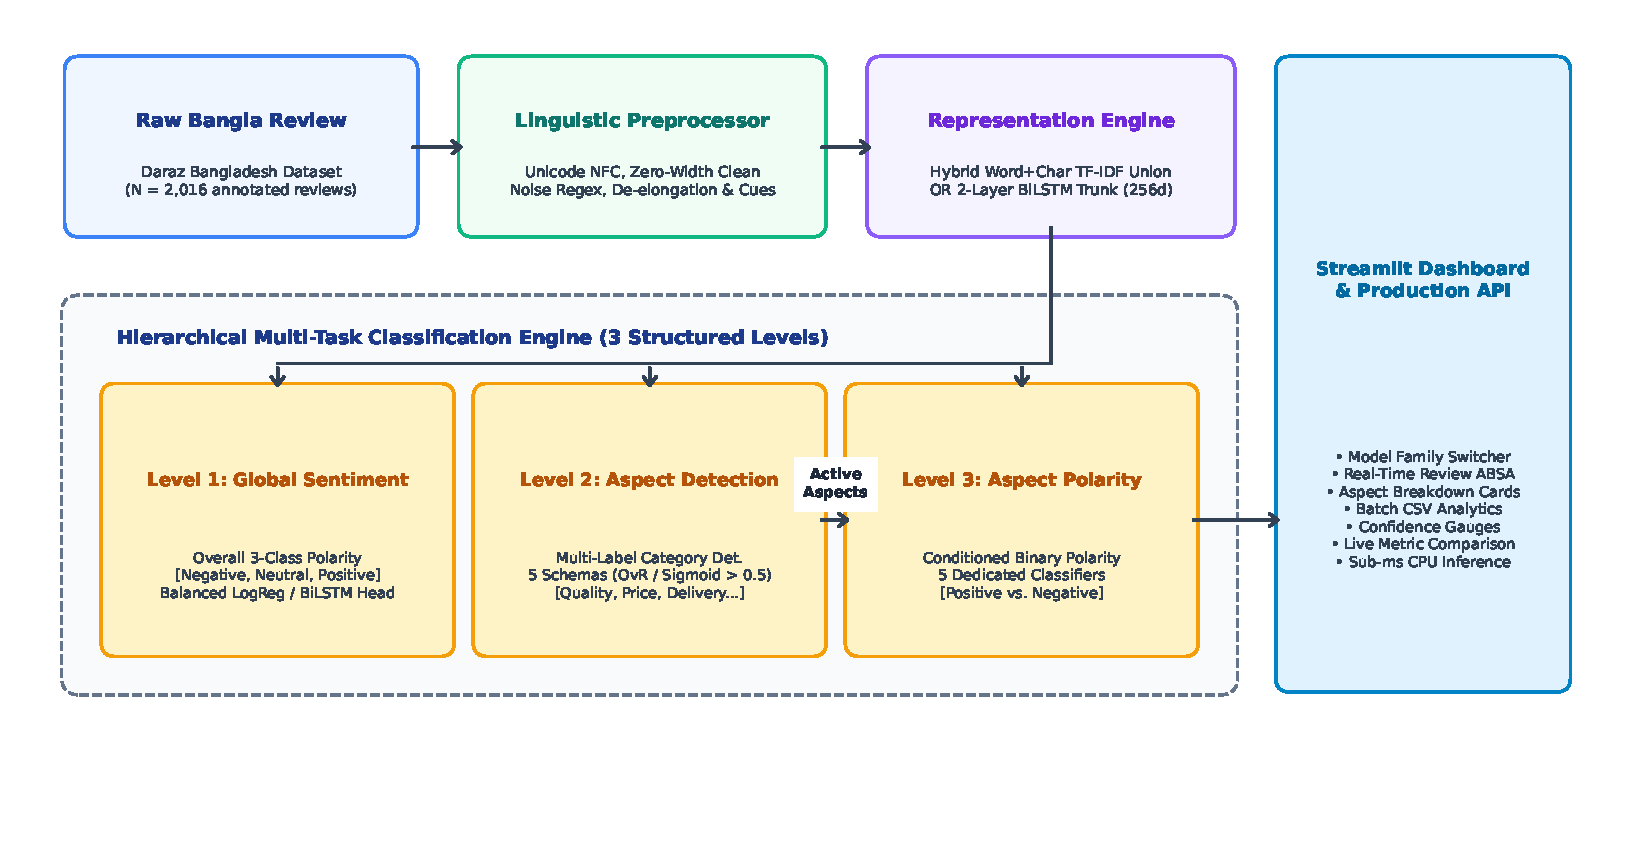
\includegraphics[width=0.98\textwidth]{figures/system_architecture.pdf}
\caption{End-to-End Hierarchical ABSA System Architecture and Workflow.}
\label{fig:sys_arch}
\end{figure}

\subsection{Hierarchical 3-Level Decision Pipeline}
Let an input Bangla review be a token sequence $T = (w_1, w_2, \dots, w_m)$. The inference pipeline executes across three structured tiers:
\begin{itemize}
    \item \textbf{Level 1: Global Sentiment Classification.} Predict the overall document polarity $y_{\mathrm{sent}} \in \{\mathrm{Negative}, \mathrm{Neutral}, \mathrm{Positive}\}$.
    
    \item \textbf{Level 2: Multi-Label Aspect Category Detection.} Identify all aspect categories discussed in review $T$ from a schema of $K = 5$ core dimensions:
    \begin{equation}
        \mathcal{A} = \{\mathrm{Product\ Quality}, \mathrm{Price}, \mathrm{Delivery}, \mathrm{Packaging}, \mathrm{Seller\ Service}\}
    \end{equation}
    The target is formalized as a binary indicator vector $\mathbf{a} = [a_1, a_2, \dots, a_K]^T \in \{0, 1\}^K$ evaluated against a decision threshold $\tau = 0.5$.
    
    \item \textbf{Level 3: Aspect-Specific Polarity Classification.} For each active aspect category $k$ satisfying $a_k = 1$, predict its specific polarity $p_k \in \{\mathrm{Negative}, \mathrm{Positive}\}$. Aspects not detected in Level 2 are skipped, ensuring computational efficiency and eliminating false-positive polarity predictions.
\end{itemize}

% =========================================================================
% 3. BANGLA PREPROCESSING METHODOLOGY
% =========================================================================
\section{Specialized Bangla Preprocessing Methodology}
\label{sec:preprocessing}

To handle informal orthography and noisy user feedback in e-commerce reviews, we construct a deterministic, 5-stage preprocessing pipeline implemented in \texttt{src/preprocessing.py}, shown in Figure~\ref{fig:preproc_flow}.

\begin{figure}[htbp]
\centering
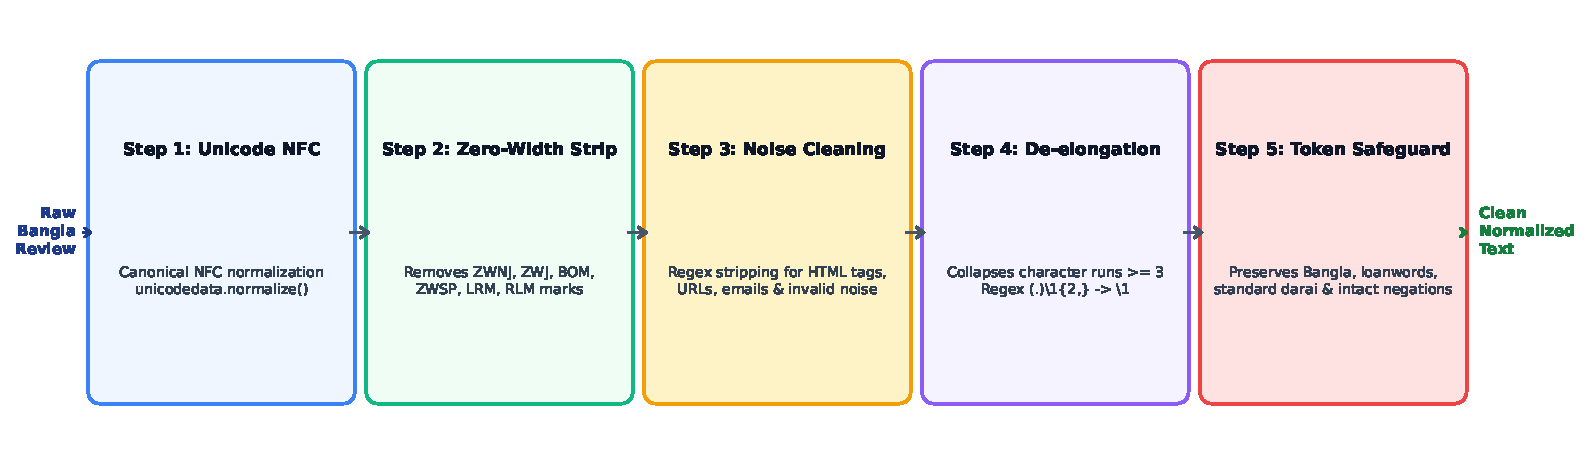
\includegraphics[width=0.98\textwidth]{figures/preprocessing_pipeline.pdf}
\caption{The 5-Stage Specialized Bangla Linguistic Preprocessing Pipeline.}
\label{fig:preproc_flow}
\end{figure}

\subsection{Step-by-Step Preprocessing Mechanisms}
\begin{enumerate}
    \item \textbf{Unicode NFC Normalization:} Text is canonicalized into Unicode Normalization Form C (NFC) via \texttt{unicodedata.normalize}, resolving disparate Unicode encodings for composite graphemes and vowel diacritics.
    
    \item \textbf{Zero-Width Character Stripping:} Invisible artifacts including Zero-Width Non-Joiners (ZWNJ, \textit{U+200C}), Zero-Width Joiners (ZWJ, \textit{U+200D}), Byte Order Marks (\textit{U+FEFF}), Zero-Width Spaces (\textit{U+200B}), and directional marks (\textit{U+200E}, \textit{U+200F}) are stripped using fast string translation tables.

    \item \textbf{Noise and Web Artifact Cleansing:} Pre-compiled regular expressions eliminate HTML markup (\verb|<[^>]+>|), HTTP/HTTPS URLs, email addresses, and non-standard symbols.
    
    \item \textbf{Character Run De-elongation:} Expressive vowel or consonant prolongations of length $\ge 3$ are collapsed to a single character using the regular expression \verb|(.)\1{2,}| $\to$ \verb|\1| (e.g., \textit{``khuuub''} $\to$ \textit{``khub''}, \textit{``onekbbb''} $\to$ \textit{``onekb''}), curbing vocabulary explosion.

    \item \textbf{Token and Negation Safeguards:} The pipeline explicitly preserves the Bangla Unicode script range (\verb|\u0980-\u09FF|), English alphanumeric tokens (\verb|A-Za-z0-9|) for code-mixed brand and model names, Bengali punctuation (\textit{darai} \verb|||), and critical polarity negation cues (\textit{na}, \textit{nai}, \textit{nei}, \textit{noy}, \textit{kintu}) to prevent polarity inversion errors during downstream vectorization.
\end{enumerate}

% =========================================================================
% 4. MODEL ARCHITECTURES & METHODOLOGIES
% =========================================================================
\section{Model Architectures and Methodologies}
\label{sec:models}

We benchmark two complementary modeling paradigms: a subword-enhanced linear pipeline and a deep recurrent neural network.

\subsection{Pipeline 1: Hybrid TF-IDF Feature Union + Balanced Linear Models}
To capture word-level semantics and sub-morphemic lexical patterns, we construct a heterogeneous feature union $\mathbf{x}_{\mathrm{tfidf}} \in \mathbf{R}^{D}$ (\texttt{src/features.py}):
\begin{equation}
    \mathbf{x}_{\mathrm{tfidf}} = \left[ \mathbf{x}_{\mathrm{word}} \,\|\, \mathbf{x}_{\mathrm{char}} \right]
\end{equation}
where:
\begin{itemize}
    \item $\mathbf{x}_{\mathrm{word}}$ extracts word $n$-grams with range $(1, 2)$ matching token pattern \verb|[\u0980-\u09FFA-Za-z0-9]+| with document frequency bounds $\mathrm{df} \in [2, 0.95 \cdot N]$.
    \item $\mathbf{x}_{\mathrm{char}}$ extracts character $n$-grams within word boundaries (\texttt{char\_wb}) with range $(3, 5)$ to capture morphological affixes and stems.
    \item Sublinear term frequency scaling is applied: $\mathrm{tf}_{\mathrm{sub}} = 1 + \log(\mathrm{tf})$ for $\mathrm{tf} > 0$.
\end{itemize}

For classification, we deploy $L_2$-regularized Logistic Regression ($C = 1.0$) optimized via L-BFGS with inverse class-frequency weighting:
\begin{equation}
    \min_{\mathbf{w}, b} \frac{1}{2}\norm{\mathbf{w}}_2^2 + C \sum_{i=1}^{N} \alpha_{y_i} \ell(y_i, \mathbf{w}^T \mathbf{x}_i + b), \quad \alpha_c = \frac{N}{J \cdot N_c}
\end{equation}
where $J$ denotes the number of classes. For Level 2 multi-label aspect detection, a One-vs-Rest (OvR) scheme with $K = 5$ binary estimators is trained.

\subsection{Pipeline 2: Deep Bidirectional LSTM (BiLSTM)}
The deep sequential baseline processes token sequences through recurrent temporal representations, as shown in Figure~\ref{fig:bilstm_arch}.

\begin{figure}[htbp]
\centering
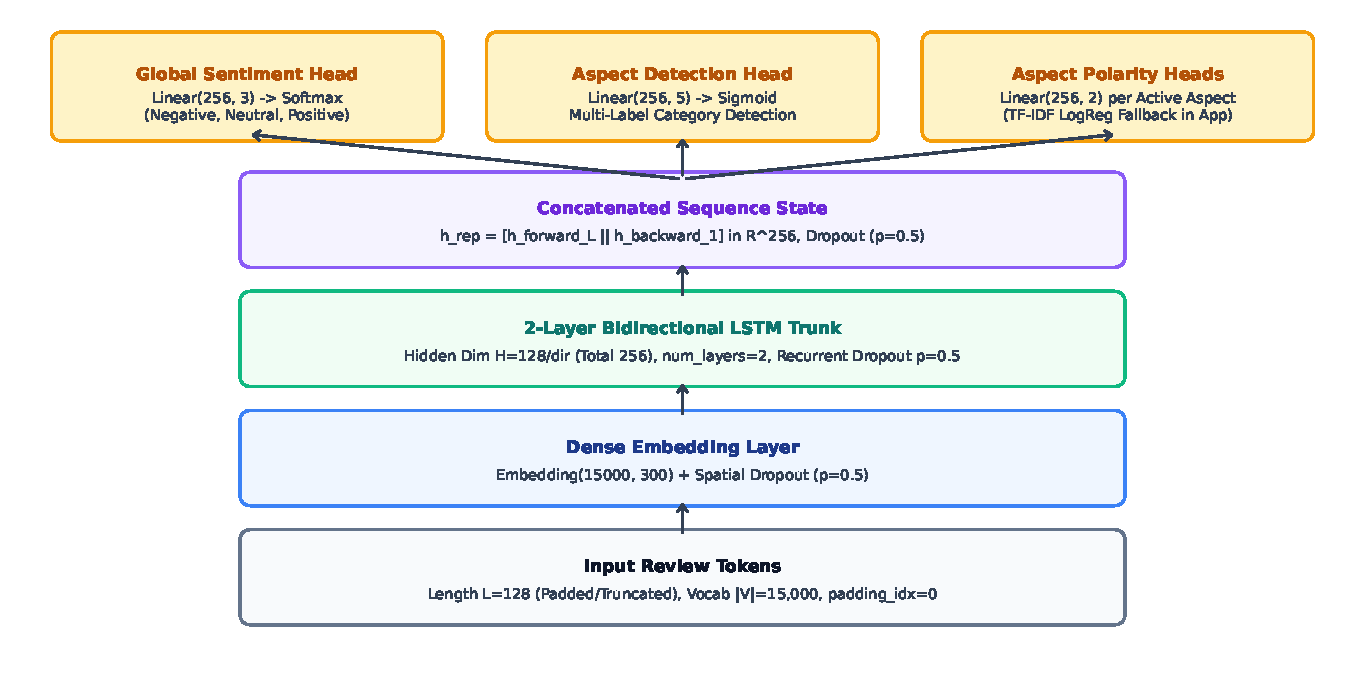
\includegraphics[width=0.88\textwidth]{figures/bilstm_architecture.pdf}
\caption{Deep Bidirectional LSTM (BiLSTM) Multi-Task Neural Network Architecture.}
\label{fig:bilstm_arch}
\end{figure}

The BiLSTM architecture (\texttt{\_LSTMBase} in \texttt{src/features.py}) comprises:
\begin{enumerate}
    \item \textbf{Vocabulary and Embedding Layer:} Sequences are padded or truncated to length $L = 128$ over a vocabulary $|\mathcal{V}| = 15{,}000$ ($\mathrm{min\_freq} = 2$) and projected into dense embeddings $\mathbf{E} \in \mathbf{R}^{|\mathcal{V}| \times d}$ ($d = 300$, \texttt{padding\_idx=0}), followed by spatial dropout ($p = 0.5$).
    
    \item \textbf{Stacked BiLSTM Trunk:} A 2-layer BiLSTM network captures bidirectional temporal dependencies:
    \begin{eqnarray}
        \vec{h}_t^{(l)} &=& \mathrm{LSTM}_{\mathrm{fwd}}^{(l)}(\mathbf{h}_t^{(l-1)}, \vec{h}_{t-1}^{(l)}) \\
        \overleftarrow{h}_t^{(l)} &=& \mathrm{LSTM}_{\mathrm{bwd}}^{(l)}(\mathbf{h}_t^{(l-1)}, \overleftarrow{h}_{t+1}^{(l)})
    \end{eqnarray}
    with hidden dimension $H = 128$ per direction (total 256 dimensions) and inter-layer dropout $p = 0.5$.
    
    \item \textbf{Sequence Representation:} The sentence representation $\mathbf{h}_{\mathrm{rep}} \in \mathbf{R}^{2H}$ concatenates the final forward and backward states: $\mathbf{h}_{\mathrm{rep}} = [ \vec{h}_L^{(2)} \,\|\, \overleftarrow{h}_1^{(2)} ]$, followed by a dropout layer ($p = 0.5$).
    
    \item \textbf{Task Classification Heads:}
    \begin{itemize}
        \item \textit{Global Sentiment Head (\texttt{SentimentLSTM}):} A linear layer projecting $256 \to 3$ outputs trained via Cross-Entropy loss.
        \item \textit{Aspect Detection Head (\texttt{AspectLSTM}):} A linear layer projecting $256 \to 5$ outputs trained via Binary Cross-Entropy with Logits (\texttt{BCEWithLogitsLoss}).
        \item \textit{Aspect Polarity Heads:} Binary linear heads projecting $256 \to 2$ outputs. In the production web application (\texttt{app.py}), aspect polarities leverage the tuned TF-IDF linear classifiers as the robust inference engine due to sample sparsity in low-frequency aspects.
    \end{itemize}
\end{enumerate}

Both PyTorch models are optimized using Adam ($\eta = 10^{-3}$, batch size $B = 32$, 10 epochs).

% =========================================================================
% 5. EXPERIMENTAL RESULTS & EVALUATION
% =========================================================================
\section{Experimental Results and Empirical Evaluation}
\label{sec:results}

\subsection{Dataset Partitioning}
The empirical benchmark was conducted on $N = 2{,}016$ labeled Bangla reviews from Daraz Bangladesh, partitioned using a stratified split (Seed = 42):
\begin{itemize}
    \item \textbf{Training Set:} $N_{\mathrm{train}} = 1{,}612$ ($80\%$)
    \item \textbf{Held-Out Test Set:} $N_{\mathrm{test}} = 404$ ($20\%$)
\end{itemize}

\subsection{Quantitative Performance Comparison}
Table~\ref{tab:results} presents the quantitative benchmark results recorded across all three hierarchical levels on the test partition.

\begin{table}[htbp]
\centering
\caption{Comprehensive performance comparison across all hierarchical tasks on the test set ($N_{\mathrm{test}} = 404$).}
\label{tab:results}
\vspace{0.3cm}
\begin{tabular}{llcccc}
\hline\hline
\textbf{Task / Target} & \textbf{Architecture} & \textbf{Accuracy} & \textbf{Macro-F1} & \textbf{Weighted-F1} & \textbf{Diagnostic Metric} \\
\hline
\multirow{2}{*}{\textbf{Global Sentiment}} 
    & \textbf{TF-IDF + LogReg} & \textbf{0.9158} & \textbf{0.8490} & \textbf{0.9197} & -- \\
    & PyTorch BiLSTM           & 0.8886          & 0.7846          & 0.8874          & -- \\
\hline
\multirow{2}{*}{\textbf{Aspect Detection}} 
    & \textbf{TF-IDF + OvR}    & \textbf{0.9644} & \textbf{0.8038} & \textbf{0.9376} & Micro-F1: \textbf{0.9364} \\
    & PyTorch BiLSTM           & 0.9609          & 0.4986          & 0.9048          & Micro-F1: 0.9281 \\
\hline
\multicolumn{6}{l}{\textbf{Aspect Polarity Classification:}} \\
\textit{Product Quality} & \textbf{TF-IDF + LogReg} & \textbf{0.9725} & \textbf{0.9514} & \textbf{0.9729} & $N_{\mathrm{train}} = 1{,}452$ \\
                        & PyTorch BiLSTM           & 0.9615          & 0.9292          & 0.9613          & $N_{\mathrm{train}} = 1{,}452$ \\
\hline
\textit{Price}           & \textbf{TF-IDF + LogReg} & \textbf{0.9789} & \textbf{0.7446} & \textbf{0.9738} & $N_{\mathrm{train}} = 376$ \\
                        & PyTorch BiLSTM           & 0.9474          & 0.6292          & 0.9510          & $N_{\mathrm{train}} = 376$ \\
\hline
\textit{Delivery}        & \textbf{TF-IDF + LogReg} & \textbf{0.8772} & \textbf{0.7580} & \textbf{0.8683} & $N_{\mathrm{train}} = 225$ \\
                        & PyTorch BiLSTM           & 0.8070          & 0.5778          & 0.7797          & $N_{\mathrm{train}} = 225$ \\
\hline
\textit{Packaging}       & \textbf{TF-IDF + LogReg} & \textbf{0.8000} & \textbf{0.7205} & \textbf{0.7702} & $N_{\mathrm{train}} = 57$ \\
                        & PyTorch BiLSTM           & 0.6667          & 0.4000          & 0.5333          & $N_{\mathrm{train}} = 57$ \\
\hline
\textit{Seller Service}  & \textbf{TF-IDF + LogReg} & \textbf{0.9545} & \textbf{0.4884} & \textbf{0.9323} & $N_{\mathrm{train}} = 86$ \\
                        & PyTorch BiLSTM           & \textbf{0.9545} & 0.4884          & 0.9323          & $N_{\mathrm{train}} = 86$ \\
\hline\hline
\end{tabular}
\end{table}

\subsection{Key Findings and Discussion}
\begin{enumerate}
    \item \textbf{Superiority of Subword Character $n$-Grams:} The hybrid TF-IDF linear pipeline outperforms the BiLSTM architecture across all tasks, attaining higher global sentiment accuracy ($91.58\%$ vs.\ $88.86\%$) and superior sentiment Macro-F1 ($0.8490$ vs.\ $0.7846$). The character $n$-gram feature union ($3 \le n \le 5$) directly captures sub-morphemic roots and negation affixes without requiring large pretraining corpora.
    
    \item \textbf{Data Scarcity in Neural Sequential Models:} The BiLSTM architecture, training embeddings from scratch on $N_{\mathrm{train}} = 1{,}612$ samples, exhibits diminished recall on rare categories (aspect detection Macro-F1 of $0.4986$ vs.\ $0.8038$ for TF-IDF). Its unconstrained parameter space suffers from sample scarcity compared to class-weighted convex linear models.
    
    \item \textbf{Aspect Polarity Dynamics:} On high-support aspects such as \textit{Product Quality} ($N_{\mathrm{train}} = 1{,}452$), both models demonstrate high accuracy ($97.25\%$ vs.\ $96.15\%$). On rare aspects such as \textit{Packaging} ($N_{\mathrm{train}} = 57$), TF-IDF achieves substantially higher Macro-F1 ($0.7205$ vs.\ $0.4000$).
    
    \item \textbf{Computational Efficiency:} The TF-IDF linear pipeline delivers sub-millisecond CPU inference per review, making it optimal for lightweight, production web deployment.
\end{enumerate}

% =========================================================================
% 6. SYSTEM IMPLEMENTATION & DEPLOYMENT
% =========================================================================
\section{System Implementation and Deployment}
\label{sec:system}

The codebase is structured into modular Python components with clear separation of responsibilities:
\begin{itemize}\setlength{\itemsep}{0.5pt}\setlength{\parsep}{0pt}
    \item \texttt{src/config.py}: Central configuration constants, hyperparameter definitions, and path mappings.
    \item \texttt{src/preprocessing.py}: High-throughput 5-stage Unicode normalization, regex de-elongation, and token safeguards.
    \item \texttt{src/data\_processing.py}: Dataset ingestion, multi-delimiter label parsing (\verb|#| and \verb|;|), and stratified splitting.
    \item \texttt{src/features.py}: Heterogeneous TF-IDF FeatureUnion and PyTorch \texttt{BanglaVocab} and \texttt{\_LSTMBase} networks.
    \item \texttt{src/train.py} \& \texttt{src/evaluate.py}: Automated multi-tier model training, evaluation metrics, and benchmark exports.
    \item \texttt{src/persistence.py}: Serialization and deserialization for TF-IDF (\texttt{.pkl}) and PyTorch (\texttt{.pt}) models.
    \item \texttt{src/predict.py}: Unified inference orchestrator bundling preprocessing and hierarchical ABSA inference.
    \item \texttt{app.py}: Production Streamlit dashboard with model switching, real-time diagnostics, and batch CSV analysis.
\end{itemize}

% =========================================================================
% 7. CONCLUSION
% =========================================================================
\section{Conclusion}
\label{sec:conclusion}

This project presented an end-to-end, methodology-focused realization of Hierarchical Aspect-Based Sentiment Analysis on Bangla e-commerce customer reviews. By combining domain-tailored linguistic preprocessing (Unicode canonicalization, zero-width stripping, character de-elongation, and negation safeguards) with a hybrid TF-IDF feature union and class-weighted linear models, our system achieves $91.58\%$ sentiment accuracy and a $0.9364$ aspect Micro-F1. The resulting modular pipeline and interactive Streamlit web platform deliver efficient, actionable review analytics for e-commerce merchants.

\end{document}
